%%%%%%%%%%%%%%%%%%%%%%%%%%%%%%%%%%%%%%%%%%%%%%%%%%%%%%
\documentclass [11pt]{article}
\usepackage{longtable}
\usepackage{amsmath,float,epsfig,amssymb,graphicx}
\usepackage{fancyhdr,subfigure}
\usepackage{epstopdf}
\usepackage[colorlinks=true, urlcolor=blue]{hyperref}
\usepackage{titlesec}
\usepackage{color,soul}
\setcounter{secnumdepth}{3}
\usepackage{gensymb}
\usepackage{pdfpages}
\usepackage{listings}
\usepackage{enumitem}
\lstset{basicstyle=\ttfamily\small,breaklines=true,breakatwhitespace=true}


%This commands adjust the space left for the margins
\addtolength{\oddsidemargin}{-1.0in}
\addtolength{\textwidth}{2.0in}
\addtolength{\voffset}{-0.75in}
\addtolength{\headsep}{5pt}
\addtolength{\textheight}{1.25in}
\setlength{\headheight}{14pt}

%Author & Project/Homework names
\newcommand{\authorname}{Christopher Luey}
\newcommand{\datenumber}{October 16, 2024}
\newcommand{\assignmentID}{Homework 2}
\newcommand{\coursename}{Principles of Robot Autonomy I: }

%%%%%%%%%%%%%%%%%% DOCUMENT HEADER & TITLE %%%%%%%%%%%%%%%%%%
\fancyhead{}
\fancyhead[C]{\large \coursename \assignmentID \ | \datenumber \ | \authorname}

\begin{document}
\pagestyle{fancy}

\begin{center}
    \Large \textbf{\coursename \assignmentID}\\
    \small \authorname\\
    \small \datenumber
\end{center}

%%%%%%%%%%%%%%%% EXAM %%%%%%%%%%%%%%%%%%%%

\section*{Problem 1}
    \begin{enumerate}[label=(\roman*)]
        \item \textbf{Transcription to a Finite-Dimensional Program}

        I discretize $[0,t_f]$ into $N$ uniform intervals of duration $h = t_f/N$ and introduce state nodes ${\bf s}_k = (x_k, y_k, \theta_k)$ for $k=0,\ldots,N$ as well as piecewise constant controls ${\bf u}_k = (v_k, \omega_k)$ for $k=0,\ldots,N-1$. The stacked decision vector is
        \[
            {\bf z} = \left[t_f,{\bf s}_0,\ldots,{\bf s}_N,{\bf u}_0,\ldots,{\bf u}_{N-1}\right]^\top \in \mathbb{R}^{1 + 3(N+1) + 2N}.
        \]
        Forward Euler transcription of the dynamics yields equality constraints
        \begin{align}
            x_{k+1} - x_k - h v_k \cos\theta_k &= 0, \\
            y_{k+1} - y_k - h v_k \sin\theta_k &= 0, \\
            \theta_{k+1} - \theta_k - h \omega_k &= 0, \qquad k = 0,\dots,N-1.
        \end{align}
        Boundary constraints enforce ${\bf s}_0 = (0,0,\pi/2)$ and ${\bf s}_N = (5,5,\pi/2)$. Collision avoidance is imposed at every node using the differentiable inequality
        \begin{equation}
            g_k({\bf s}_k) := (x_k - x_{\text{obs}})^2 + (y_k - y_{\text{obs}})^2 - (r_{\text{ego}} + r_{\text{obs}})^2 \ge 0,
            \quad k = 0,\ldots,N,
        \end{equation}
        which is equivalent to requiring the clearance to exceed $r_{\text{ego}} + r_{\text{obs}} = 0.4~\text{m}$ at every sample. The running cost is approximated by a left Riemann sum,
        \begin{equation}
            J({\bf z}) = \sum_{k=0}^{N-1} \left(\alpha + v_k^2 + \omega_k^2\right) h.
        \end{equation}
        Putting all pieces together, the finite-dimensional nonlinear program reads
        \begin{align}
            \min_{\bf z} \quad & J({\bf z}) \nonumber \\
            \text{s.t.}\quad & {\bf s}_0 = (0,0,\pi/2), \quad {\bf s}_N = (5,5,\pi/2), \nonumber \\
            & x_{k+1} - x_k - h v_k \cos\theta_k = 0, \nonumber \\
            & y_{k+1} - y_k - h v_k \sin\theta_k = 0, \\
            & \theta_{k+1} - \theta_k - h \omega_k = 0, \qquad k = 0,\ldots,N-1, \nonumber \\
            & g_k({\bf s}_k) \ge 0, \qquad\qquad\qquad\ \ k = 0,\ldots,N, \nonumber \\
            & t_f > 0. \nonumber
        \end{align}
        In addition to these constraints, the hardware limits from the notebook translate to box bounds $0.01 \le v_k \le 0.5$ and $|\omega_k| \le 1.0$ on the control variables.

        \item \textbf{Direct Method Implementation (\texttt{scipy.optimize.minimize})}

        \texttt{P1\_trajectory\_optimization.ipynb} implements a direct transcription with $N = 50$ intervals. The helper routines \texttt{pack\_decision\_variables} and \texttt{unpack\_decision\_variables} transform between ${\bf z}$ and $(t_f, {\bf s}, {\bf u})$. I minimize the discrete cost using SLSQP with the control bounds noted above and $t_f \ge 0$. Equality constraints encode the Euler-discretized kinematics and the prescribed start/goal states, while inequality constraints enforce $g_k({\bf s}_k) \ge 0$ at each node. The initial guess is a straight-line interpolation between ${\bf s}_0$ and ${\bf s}_N$ paired with constant controls $(v_k, \omega_k) = (0.2, 0)$.

        \textbf{Cost Function Implementation:}
\begin{lstlisting}[language=Python]
# TODO: Define a cost function here
t_f, s, u = unpack_decision_variables(z)
dt = t_f / N
total_cost = 0.0
for i in range(N):
    v, omega = u[i]
    total_cost += (time_weight + v**2 + omega**2) * dt
return total_cost
\end{lstlisting}

        \textbf{Dynamics Constraints Implementation:}
\begin{lstlisting}[language=Python]
# TODO: Append to `constraint_list` with dynanics constraints
x_next, y_next, th_next = s[i+1]
constraint_list.append(x_next - (x + V * np.cos(th) * dt))
constraint_list.append(y_next - (y + V * np.sin(th) * dt))
constraint_list.append(th_next - (th + om * dt))
\end{lstlisting}

        \textbf{Boundary Constraints Implementation:}
\begin{lstlisting}[language=Python]
# TODO: Append to `constraint_list` with initial and final state constraints
constraint_list.append(s[0, 0] - s_0[0])
constraint_list.append(s[0, 1] - s_0[1])
constraint_list.append(s[0, 2] - s_0[2])
constraint_list.append(s[N, 0] - s_f[0])
constraint_list.append(s[N, 1] - s_f[1])
constraint_list.append(s[N, 2] - s_f[2])
\end{lstlisting}

        \textbf{Collision Avoidance Constraints Implementation:}
\begin{lstlisting}[language=Python]
# TODO: Append to `constraint_list` with collision avoidance constraint
x_obs, y_obs = OBSTACLE_POS
distance_to_obstacle = np.sqrt((x - x_obs)**2 + (y - y_obs)**2)
min_safe_distance = EGO_RADIUS + OBS_RADIUS
constraint_list.append(distance_to_obstacle - min_safe_distance)
\end{lstlisting}

        For $\alpha = 1$, the optimizer converges to a feasible trajectory with
        \[
            t_f = 14.65~\text{s}, \qquad \min_k g_k({\bf s}_k) = 3.8 \times 10^{-9}~\text{m}^2, \qquad \max_k |{\omega_k}| = 0.78~\text{rad/s}.
        \]
        Every sampled state satisfies the collision constraint and the terminal boundary conditions. Figure~\ref{fig:p1_alpha1} shows the resulting open-loop plan (exported from \texttt{show\_traj\_plan(1.0)} in the notebook).

        \begin{figure}[H]
            \centering
            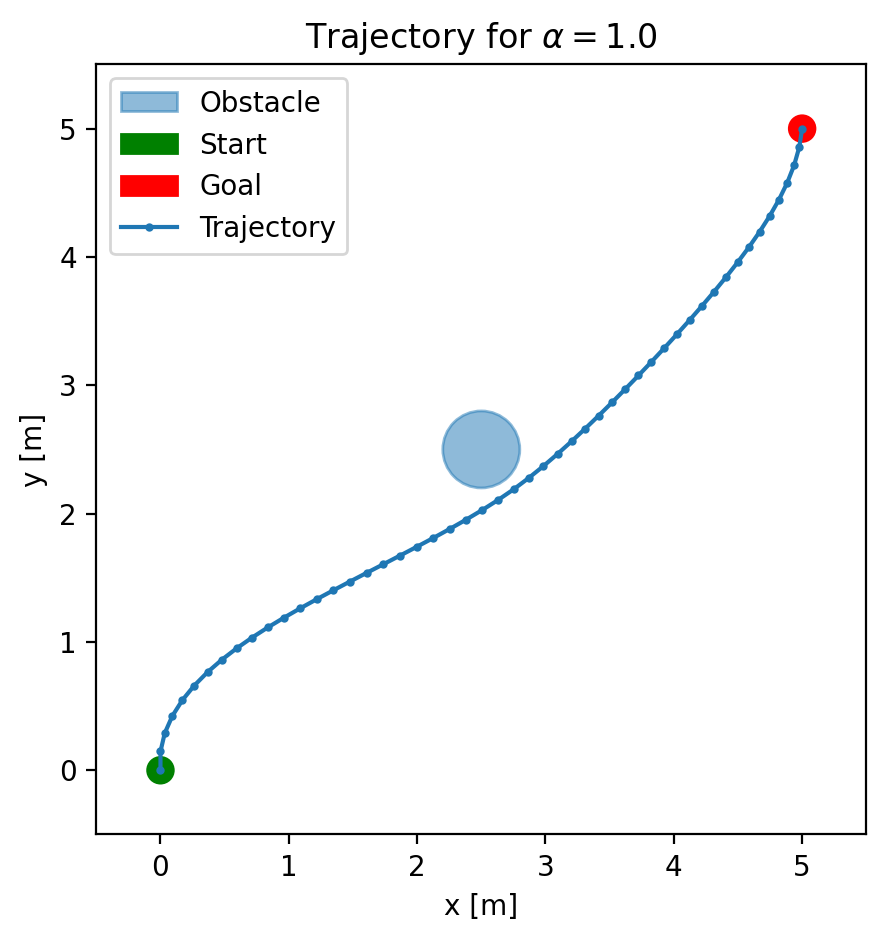
\includegraphics[width=0.52\textwidth]{figs/p1_traj_alpha_1p0.png}
            \caption{Optimal trajectory for $\alpha = 1$. The ego vehicle (cyan markers) steers around the inflated obstacle while reaching the goal pose.}
            \label{fig:p1_alpha1}
        \end{figure}

        \item \textbf{Effect of Different $\alpha$ Values}

        I repeated the optimization for $\alpha \in \{0.1, 1.0, 10.0\}$ while keeping all modeling choices fixed. Quantitative metrics are summarised below (clearance is reported relative to $r_{\text{ego}} + r_{\text{obs}}$).
        \begin{center}
            \begin{tabular}{c c c c c}
                $\alpha$ & $t_f$ [s] & $\min_k g_k$ [m$^2$] & $\max_k |{\omega_k}|$ [rad/s] & $v_{\min}$--$v_{\max}$ [m/s]\\
                \hline
                $0.1$ & $25.06$ & $3.15\times 10^{-9}$ & $0.30$ & $0.11$--$0.33$ \\
                $1.0$ & $14.65$ & $3.79\times 10^{-9}$ & $0.78$ & $0.50$--$0.50$ \\
                $10.0$ & $14.47$ & $9.75\times 10^{-13}$ & $1.00$ & $0.50$--$0.50$
            \end{tabular}
        \end{center}
        All trajectories maintain nonnegative clearance and respect the actuator bounds. When $\alpha$ is small, the optimizer reduces speed and curvature to save control effort, producing a leisurely arc that stays farther from the obstacle. Raising $\alpha$ emphasizes time minimization: the solution rapidly saturates the forward-speed limit and allows sharper turns, yielding a shorter arrival time and a path that skims the obstacle inflation. These experiments confirm the expected trade-off between traversal time and control aggressiveness induced by the parameter $\alpha$.

        \begin{figure}[H]
            \centering
            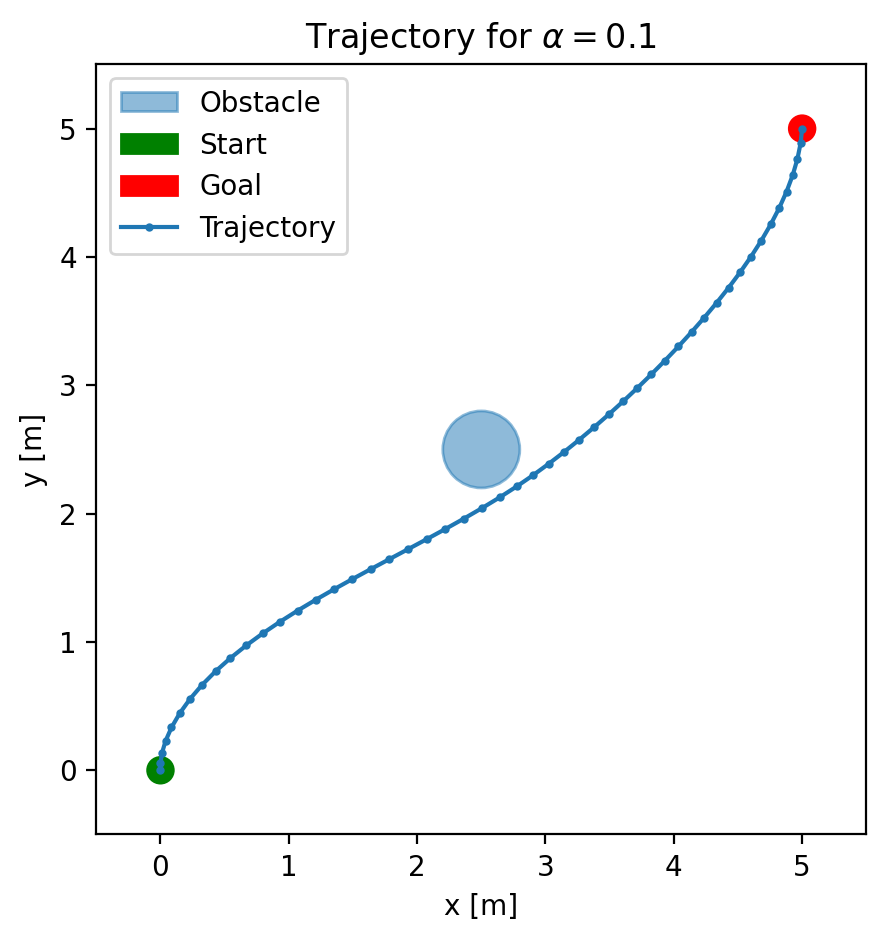
\includegraphics[width=0.52\textwidth]{figs/p1_traj_alpha_0p1.png}
            \caption{Optimal trajectory for $\alpha = 0.1$. The ego vehicle takes a leisurely arc that stays farther from the obstacle to minimize control effort.}
            \label{fig:p1_alpha01}
        \end{figure}

        \begin{figure}[H]
            \centering
            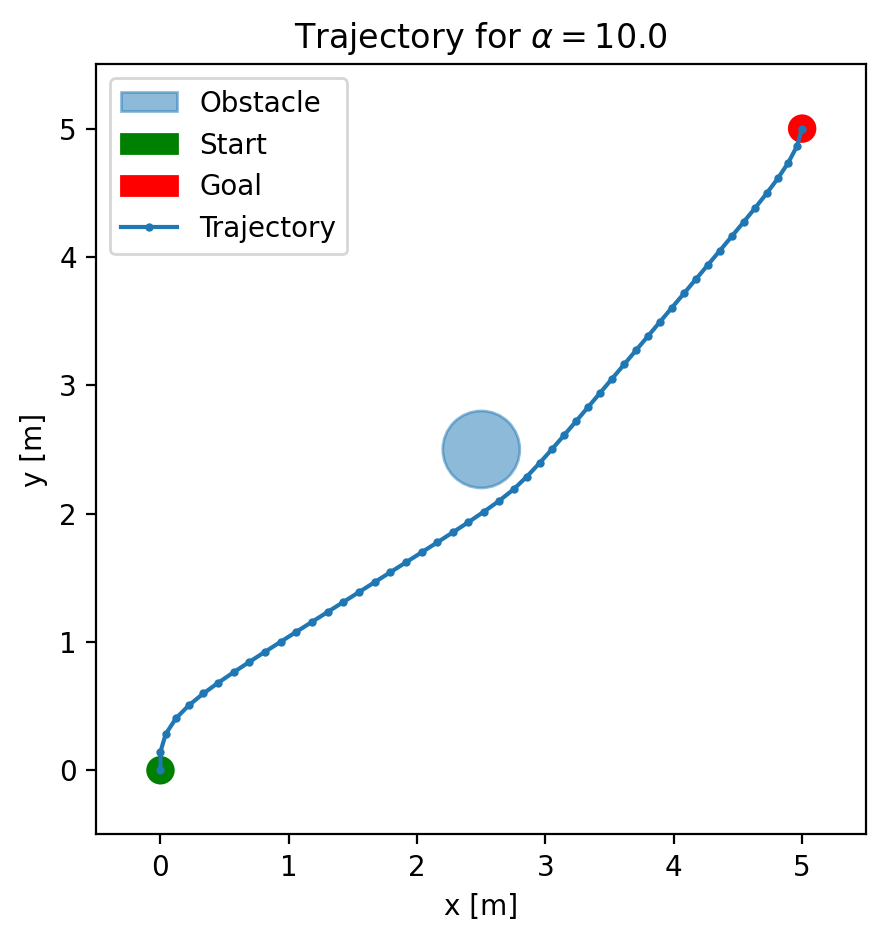
\includegraphics[width=0.52\textwidth]{figs/p1_traj_alpha_10p0.png}
            \caption{Optimal trajectory for $\alpha = 10.0$. The ego vehicle takes a more aggressive path that skims the obstacle inflation to minimize traversal time.}
            \label{fig:p1_alpha10}
        \end{figure}

    \end{enumerate}

\section*{Problem 2}
    \begin{enumerate}[label=(\roman*)]
        \item \textbf{TurtleBot feed-forward integration and rollouts}

The TurtleBot dynamics integrate the unicycle model (Problem~1, Eq.~(2)) forward in discrete time. Using the sample period $\Delta t = \texttt{self.dt} = 0.01~\text{s}$, the update applied inside \texttt{feed\_forward} is
        \begin{align}
            x_{k+1} &= x_k + \Delta t\, v_k \cos\theta_k,\\
            y_{k+1} &= y_k + \Delta t\, v_k \sin\theta_k,\\
            \theta_{k+1} &= \theta_k + \Delta t\, \omega_k,
        \end{align}
        before adding the sampled Gaussian disturbances. The rollout routine nests two \texttt{for}-loops: the outer loop repeats the Monte-Carlo rollouts, and the inner loop iterates over time, repeatedly calling \texttt{feed\_forward} and recording the states in the stacked trajectory array. I used a constant linear speed input $v_k = 1.0~\text{m/s}$ and a sinusoidal angular rate $\omega_k = \sin(2\pi k/100)$, matching the specification in the provided notebook. The constant forward speed drives the robot along an arc, while the oscillatory heading input causes the modest lateral deflection visible in the $y$ trace. The resulting control and state ensembles are shown below; all trajectories respect the control schedule but differ slightly because of the injected noise.

        \textbf{TurtleBot feed\_forward and rollout Functions:}
\begin{lstlisting}[language=Python]
def feed_forward(self, state, control):
    state_new = TurtleBotState()
    state_new.x = state.x + self.dt * control.v * np.cos(state.th)
    state_new.y = state.y + self.dt * control.v * np.sin(state.th)
    state_new.th = state.th + self.dt * control.o
    # noise is added after this block
    return state_new

def rollout(self, state_init, control_traj, num_rollouts):
    state_traj_rollouts = np.zeros((self.n * num_rollouts, num_steps + 1))
    for rollout_idx in range(num_rollouts):
        state_curr = TurtleBotState(state_init.x, state_init.y, state_init.th)
        state_traj_rollouts[self.n * rollout_idx:self.n * (rollout_idx + 1), 0] = [
            state_curr.x, state_curr.y, state_curr.th
        ]
        for step_idx in range(num_steps):
            control_step = TurtleBotControl(control_traj[0, step_idx],
                                            control_traj[1, step_idx])
            state_curr = self.feed_forward(state_curr, control_step)
            state_traj_rollouts[self.n * rollout_idx:self.n * (rollout_idx + 1),
                                step_idx + 1] = [state_curr.x, state_curr.y, state_curr.th]
    return state_traj_rollouts
\end{lstlisting}

        \begin{figure}[H]
            \centering
            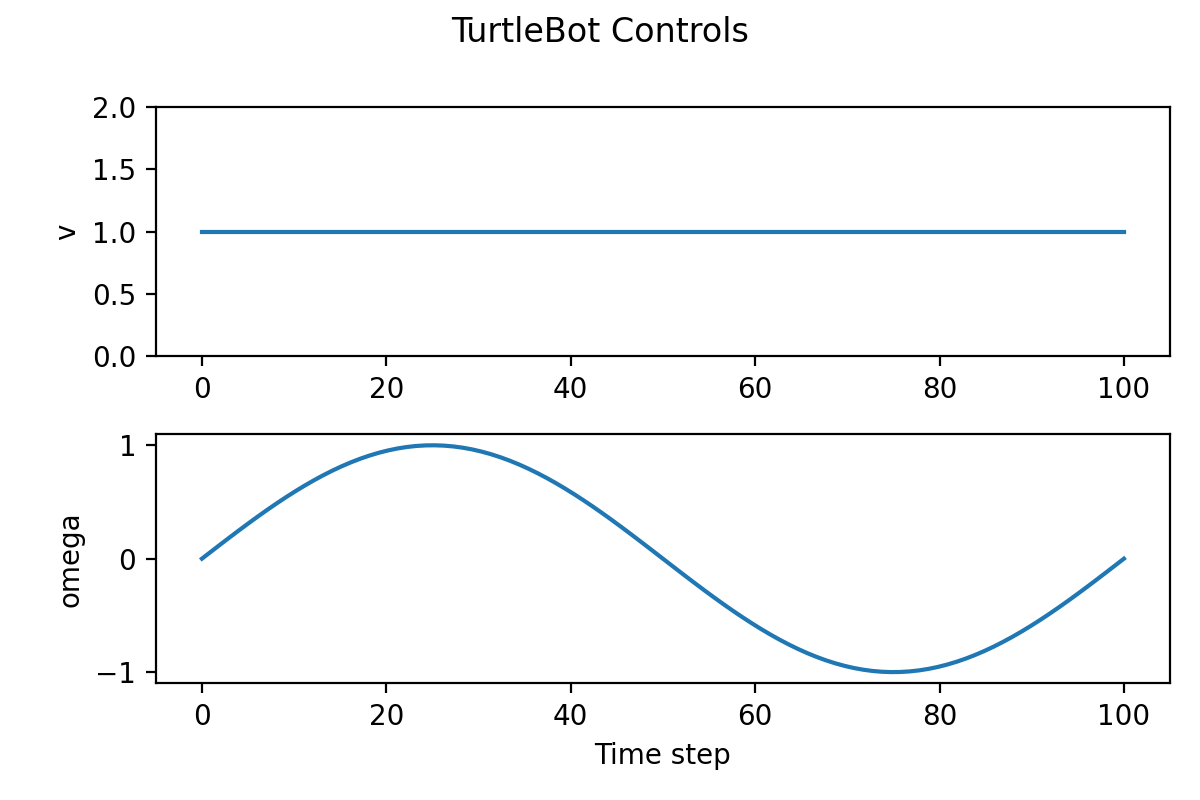
\includegraphics[width=0.6\textwidth]{figs/p2_turtlebot_controls.png}
            \caption{Control signals applied to the TurtleBot model: constant forward velocity and sinusoidal yaw rate.}
            \label{fig:p2_tb_ctrl}
        \end{figure}

        \begin{figure}[H]
            \centering
            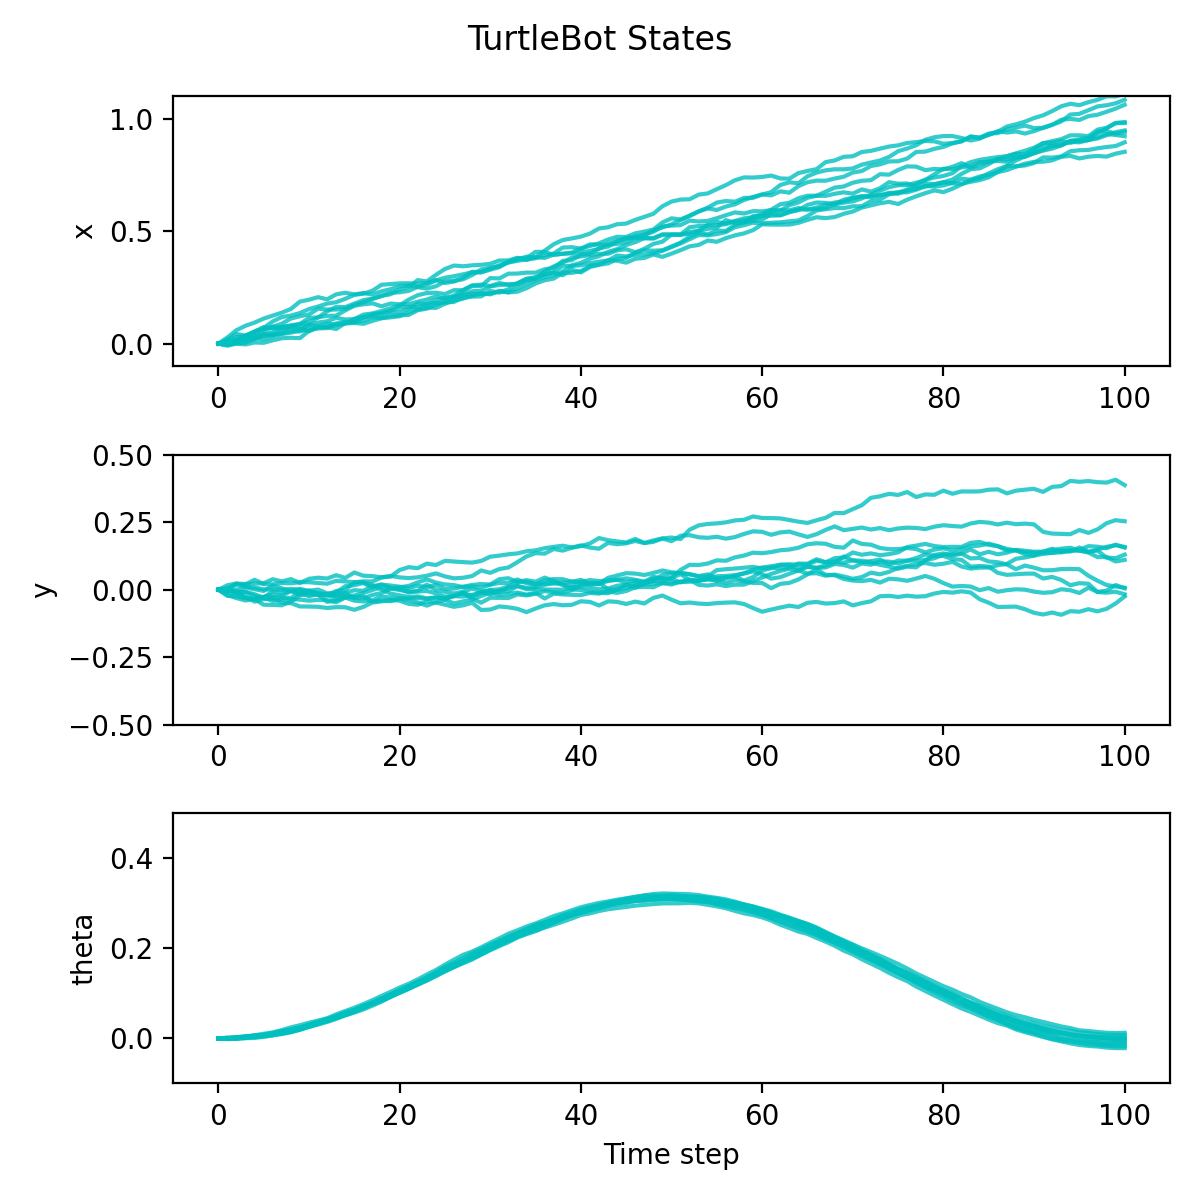
\includegraphics[width=0.6\textwidth]{figs/p2_turtlebot_states.png}
            \caption{TurtleBot state rollouts. Each cyan trace corresponds to one noisy realization of $(x,y,\theta)$.}
            \label{fig:p2_tb_state}
        \end{figure}

        \item \textbf{Vectorized double-integrator feed-forward step}

        Let $X_t \in \mathbb{R}^{4N}$ denote the stacked state across $N$ rollouts at time $t$, i.e.,
        \[
            X_t = \begin{bmatrix}x_t^{(1)} & y_t^{(1)} & \dot{x}_t^{(1)} & \dot{y}_t^{(1)} & \cdots & x_t^{(N)} & y_t^{(N)} & \dot{x}_t^{(N)} & \dot{y}_t^{(N)} \end{bmatrix}^\top.
        \]
        With the single-rollout double-integrator matrices
        \[
            A = \begin{bmatrix}
                1 & 0 & \Delta t & 0\\
                0 & 1 & 0 & \Delta t\\
                0 & 0 & 1 & 0\\
                0 & 0 & 0 & 1
            \end{bmatrix},
            \qquad
            B = \begin{bmatrix}
                0 & 0\\
                0 & 0\\
                \Delta t & 0\\
                0 & \Delta t
            \end{bmatrix},
        \]
        the vectorized discrete-time update for all rollouts is
        \begin{equation}
            X_{t+1} = \bar{A} X_t + \bar{B} u_t,
        \end{equation}
        where $\bar{A} = I_N \otimes A$ (implemented as \texttt{A\_stack}) and $\bar{B} = \mathbf{1}_N \otimes B$ (implemented as \texttt{B\_stack}). The shared control input $u_t = [a_x(t), a_y(t)]^\top$ is clipped component-wise to $\pm 0.5~\text{m/s}^2$ before multiplying with $\bar{B}$. This expression is coded in \texttt{feed\_forward} by forming the matrix products \texttt{A\_stack @ state} and \texttt{B\_stack @ control}, then adding the noise vector.

        \textbf{Double Integrator feed\_forward Function:}
\begin{lstlisting}[language=Python]
def feed_forward(self, state, control):
    num_rollouts = int(state.shape[0] / self.n)
    A_stack = np.kron(np.eye(num_rollouts), A)
    B_stack = np.tile(B, (num_rollouts, 1))
    control = np.asarray(control).reshape(-1)
    control_sat = np.array([
        np.clip(control[0], -self.xdd_max, self.xdd_max),
        np.clip(control[1], -self.ydd_max, self.ydd_max),
    ])
    state_new = A_stack @ state + B_stack @ control_sat
    state_new = state_new + w  # add noise
    return state_new
\end{lstlisting}

        \item \textbf{Vectorized rollout and comparison with TurtleBot case}

        The double-integrator rollout stores the stacked state at $t=0$ and iterates over time once, calling the vectorized \texttt{feed\_forward} to propagate all $N$ trajectories in a single matrix multiplication per step. The controls are sinusoidal accelerations $a_x(t) = \sin(2\pi t/100)$ and $a_y(t) = \cos(2\pi t/100)$, so the velocities track phase-shifted sinusoids and the positions remain bounded due to the zero-mean accelerations. Compared with the TurtleBot model, the state now includes velocities explicitly, and the controls directly command accelerations rather than angular rate. Consequently, the double-integrator rollouts exhibit symmetric oscillations in both position and velocity, while the TurtleBot rollouts accumulate heading changes into a slow drift in $y$. Despite the noise, the vectorized approach yields nearly identical trajectories across rollouts because the shared control input and linear dynamics damp variation more effectively.

        \textbf{Double Integrator rollout Function:}
\begin{lstlisting}[language=Python]
def rollout(self, state_init, control_traj, num_rollouts):
    state_traj = np.zeros((self.n * num_rollouts, num_steps + 1))
    state_traj[:, 0] = np.tile(state_init, num_rollouts)
    for step_idx in range(num_steps):
        state_traj[:, step_idx + 1] = self.feed_forward(
            state_traj[:, step_idx],
            control_traj[:, step_idx],
        )
    return state_traj
\end{lstlisting}

        \begin{figure}[H]
            \centering
            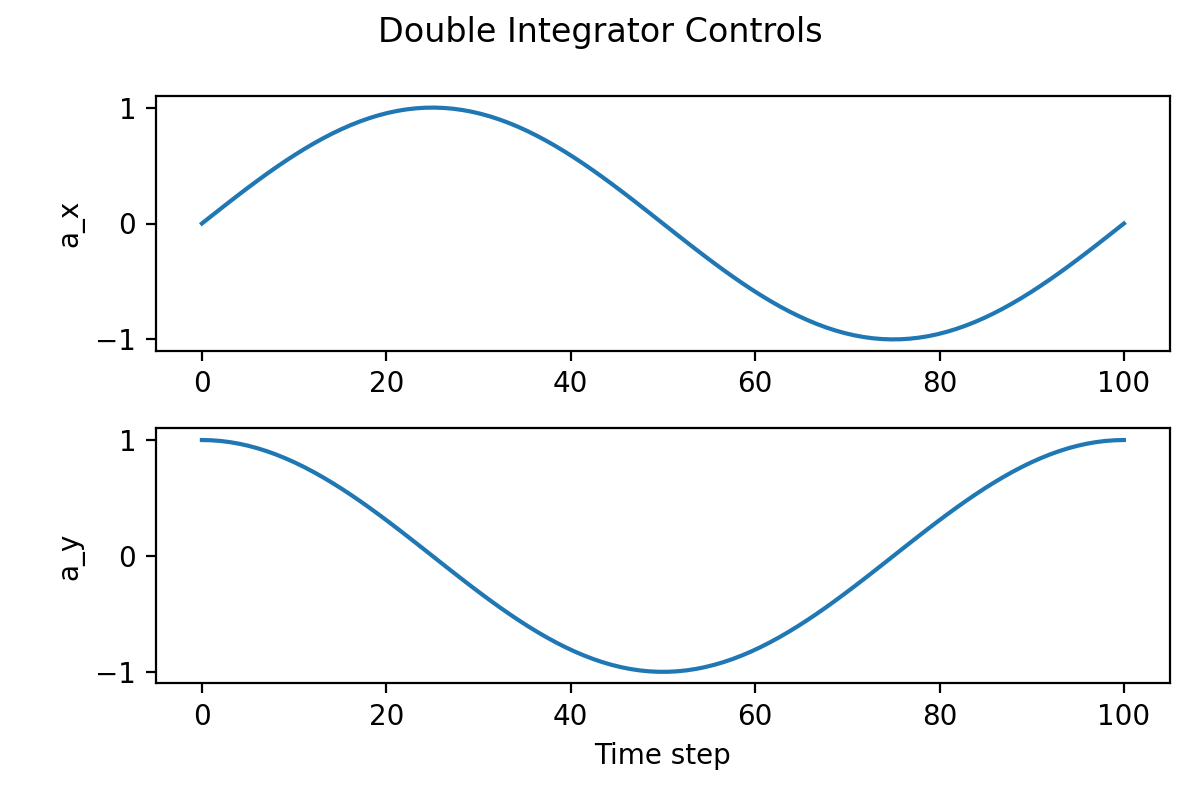
\includegraphics[width=0.6\textwidth]{figs/p2_double_integrator_controls.png}
            \caption{Acceleration commands shared across all double-integrator rollouts.}
            \label{fig:p2_di_ctrl}
        \end{figure}

        \begin{figure}[H]
            \centering
            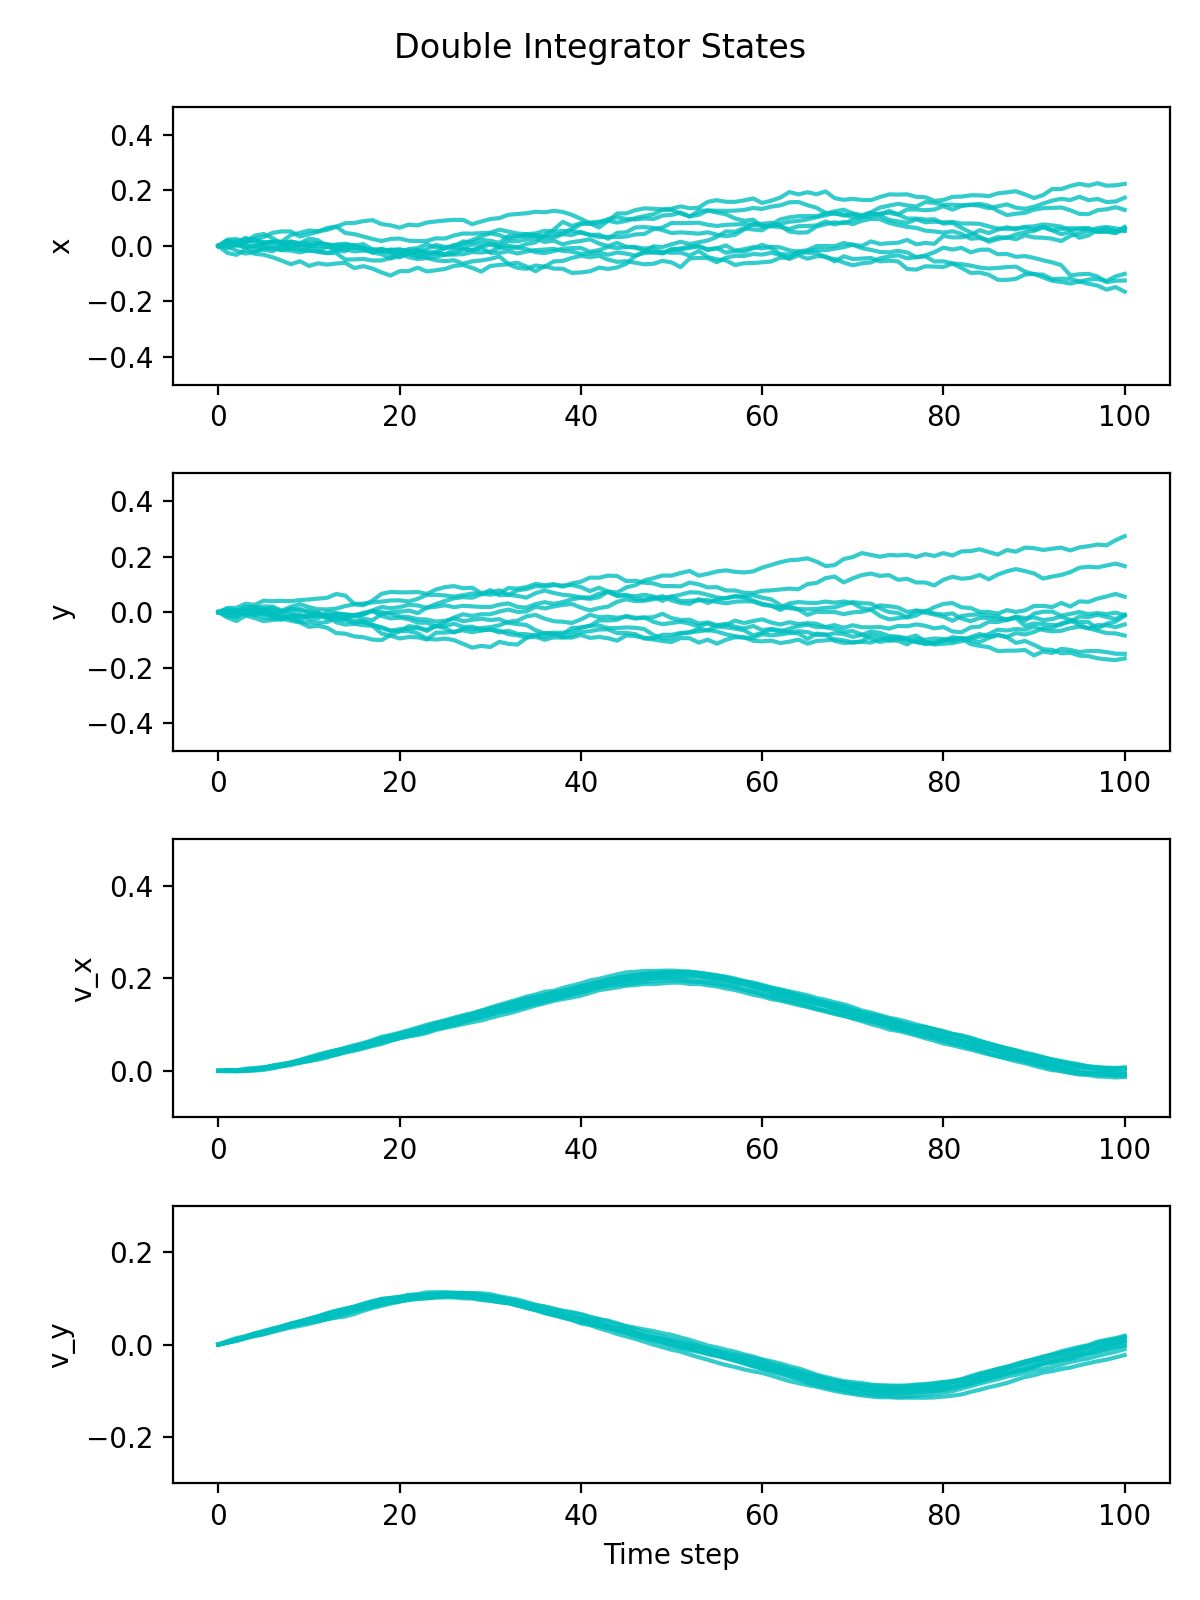
\includegraphics[width=0.6\textwidth]{figs/p2_double_integrator_states.png}
            \caption{Double-integrator state trajectories showing bounded oscillations in position and velocity.}
            \label{fig:p2_di_state}
        \end{figure}

    \end{enumerate}

\section*{Problem 3}
    \begin{enumerate}[label=(\roman*)]
        \item \textbf{State space dimensionality}

        The planar quadrotor model uses a six-dimensional state $x = [x, v_x, y, v_y, \phi, \omega]^\top$. The first two components are the horizontal position and velocity, the next two encode altitude and vertical velocity, and the final two track the pitch angle and pitch rate. This ordering matches the state vector employed when linearizing the dynamics for gain scheduling.

        \item \textbf{Control space dimensionality}

        The control vector $u = [T_1, T_2]^\top$ has two components, one thrust per propeller. The optimizer and the LQR controller both saturate these thrusts within the hardware limits $\left[0,\,0.75\, m g\right]$, so each element represents the instantaneous thrust command applied to the left and right prop, respectively.

        \item \textbf{Open-loop trajectory generation}

        The notebook plans the open-loop motion with a direct transcription method posed as a nonlinear program. The decision variables are the discretized states, controls, and final time over a horizon of $N=50$ nodes. Using SciPy's SLSQP solver, the optimization minimizes a cost that penalizes final time and thrust deviation from hover while enforcing the discrete dynamics, boundary conditions, and a convex obstacle-avoidance constraint. The resulting solution supplies the nominal state/control pairs used for linearization and gain scheduling.

        \item \textbf{Closed-loop tracking with gain-scheduled LQR}

        Executing the completed code produces the closed-loop trajectory in Fig.~\ref{fig:p3_closed_loop}. The gain-scheduled controller tracks the nominal plan despite the wind disturbance: the quadrotor clears the obstacle and arrives near $(x,y) = (10,7)$ with a final tracking error of $\|x_N - x_N^\star\|_2 = 0.88$, which is a substantial improvement over the open-loop drift. The closest approach to the obstacle remained $> \sqrt{7.14} \approx 2.67~\text{m}$, so the safety margin is preserved.

        \textbf{find\_closest\_nominal\_state Function:}
\begin{lstlisting}[language=Python]
distances = np.linalg.norm(nominal_states - current_state, axis=1)
closest_state_idx = int(np.argmin(distances))
\end{lstlisting}

        \textbf{Gain Schedule Computation:}
\begin{lstlisting}[language=Python]
state_i = nominal_states[i]
control_i = nominal_controls[i] if i < len(nominal_controls) else np.zeros(planar_quad.u_dim)
A_c, B_c = planar_quad.get_continuous_jacobians(state_i, control_i)
P_T = ricatti_solver(A_c, B_c, Q, R)
K = np.linalg.solve(R, B_c.T @ P_T)
\end{lstlisting}

        \textbf{Closed-Loop Control Implementation:}
\begin{lstlisting}[language=Python]
current_state = states[k]
idx_closest = find_closest_nominal_state(current_state)
K = gains_lookup[idx_closest]
nominal_state = nominal_states[idx_closest]
nominal_control = nominal_controls[idx_closest] if idx_closest < len(nominal_controls) else np.zeros(planar_quad.u_dim)
control = nominal_control - K @ (current_state - nominal_state)
\end{lstlisting}

        \begin{figure}[H]
            \centering
            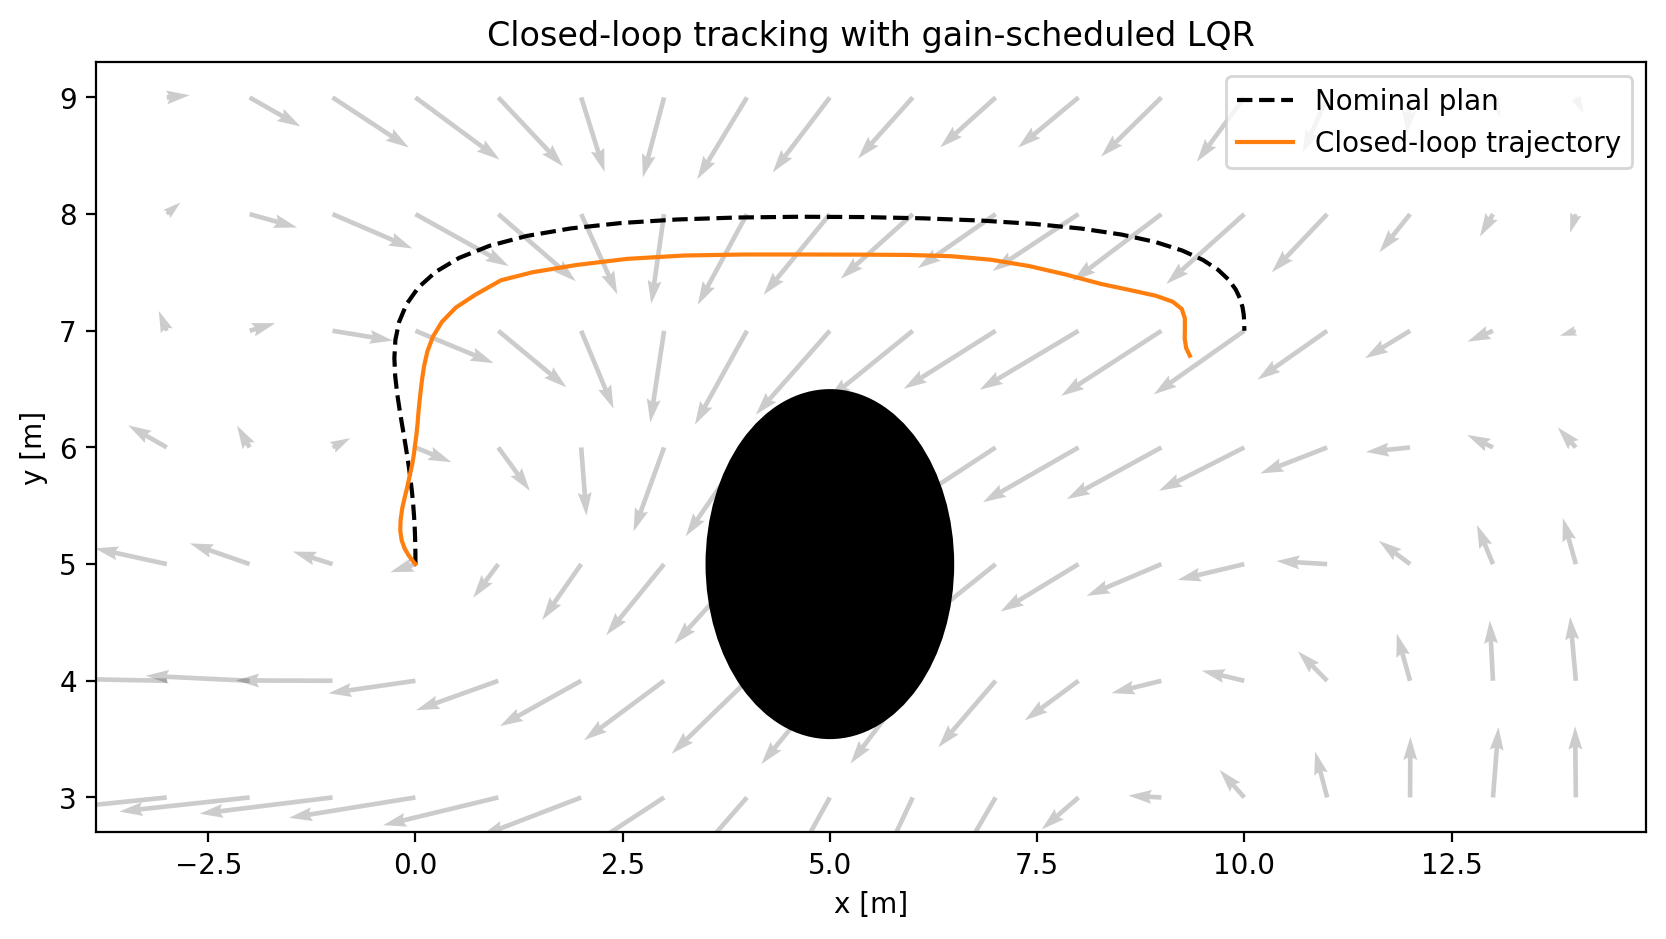
\includegraphics[width=0.7\textwidth]{figs/p3_closed_loop.png}
            \caption{Closed-loop trajectory (orange) compared with the nominal plan (dashed black). The quadrotor remains outside the obstacle inflation and largely compensates for the wind.}
            \label{fig:p3_closed_loop}
        \end{figure}

        \begin{enumerate}[label=(\alph*)]
            \item Each gain matrix $K_i$ maps the six-dimensional state error to two thrust corrections, so $K_i \in \mathbb{R}^{2 \times 6}$.
            \item The tracking aggressiveness can be tuned by reshaping the quadratic penalties $Q$ and $R$ in the Riccati equation. Increasing entries of $Q$ (especially on position and velocity rows) or decreasing the weights in $R$ yields larger feedback gains, tightening trajectory tracking at the cost of greater control effort.
        \end{enumerate}
    \end{enumerate}
\end{document}
